
\subsection{Explicación formal del problema}

Para entender mejor el problema, lo especificaremos usando términos matemáticos. Se tiene un conjunto de $n$ elementos que representan a los guerreros. 
\[G = \{g_1,...,g_n\}\]

Definiremos una \emph{partición} (\emph{pelea} en el enunciado) como un par de dos conjuntos disjuntos no vacíos de elementos $A$ y $B$ (donde cada uno representa cada bando en una pelea). En cada partición, la unión de dichos conjuntos es el conjunto total de los elementos (es decir, todos los guerreros participan de todas las peleas):
\[ P = (A, B)\]
donde $A$, $B$ son conjuntos de elementos y  \[A \ \dot{\cup}\ B = G.\]

Notaremos $P_A$ al conjunto $A$ de elementos que representa al primer elemento de la partición $P$, y $P_B$ al del otro. Además, para todo elemento $g_k$, notaremos $B_P(g_k)$ (bando, en los t\'erminos del enunciado) al conjunto de la particion $P$ al que $g_k$ pertenece. O sea que los valores que puede tomar $B_P(g_k)$ son $P_A$ o $P_B$. 

Dada una cantidad de elementos $n$, se pide encontrar el conjunto de tamaño mínimo de particiones de modo que para todo par de elementos $(g_i, g_j)$, exista particion $P$ tal que $B_P(g_i) \neq B_P(g_j)$.

ACA VAN A IR UNOS DIBUJITOS

%\begin{figure}[htbp]
%\centering
%\subfigure[Solución incorrecta]{\includegraphics[width=40mm]{}}
%\subfigure[Solución correcta]{\includegraphics[width=40mm]{}}
%\caption{Ejemplo con n=4} \label{kaioken1}
%\end{figure}
%
%\begin{figure}[htbp]
%\centering
%\subfigure[Solución incorrecta]{\includegraphics[width=40mm]{}}
%\subfigure[Solución correcta]{\includegraphics[width=40mm]{}}
%\subfigure[Solución incorrecta]{\includegraphics[width=40mm]{}}
%\subfigure[Solución correcta]{\includegraphics[width=40mm]{}}
%\caption{Ejemplo con n=7} \label{kaioken2}
%\end{figure}

Notar que puede haber más de una solución correcta. El algoritmo propuesto devuelve una de ellas.

\subsection{Explicación de la solución}

Para explicar la solución, mezclaremos el lenguaje del problema original con el lenguaje formal, usando el que creamos que hará más clara la explicación en cada momento.

Para resolver el problema, utilizamos un algoritmo usando la técnica de \textbf{divide and conquer}, es decir, dividimos el problema en subproblemas más pequeños, los resolvemos, y luego combinamos las soluciones para lograr la solución al problema total.

Para entender cómo lo aplicamos para resolver el problema, consideremos la primera partición: $P_1$, cuando todavía no comenzaron los guerreros a pelear.
Para dicha pelea, se eligen guerreros para el bando $P_{1A}$ y para el bando $P_{1B}$, de modo que luego de la pelea, todos los guerreros del bando A hubieron peleado contra los del B y viceversa.
De este modo, a los guerreros del bando A, les faltará solamente pelear entre sí, al igual que los del bando B.

Ahora bien, tenemos dos subproblemas separados: 
\begin{itemize}
\item Por un lado, necesitamos que todos los guerreros de $P_{1A}$ peleen entre sí, en la cantidad mínima de peleas posible.
\item Por otro lado, buscaremos lo mismo para los guerreros de $P_{1B}$.
\end{itemize}

Una vez resueltos estos subproblemas, la manera de combinar las soluciones es simple. Supongamos que para la siguiente pelea, los guerreros de $P_{1A}$ se dividen en dos bandos: $C$ y $D$, y los guerreros de $P_{1B}$ se dividen en los bandos $E$ y $F$. Podemos combinar la solución en una única pelea $P_2$, tomamos $P_2$ = $(C \cup E,\ D \cup F)$, de modo que en una misma pelea se logren enfrentar los guerreros de $C$ y $D$, y de $E$ y $F$. De la misma forma procedemos para las siguientes peleas.

Podría pasar que cuando aplicamos el algoritmo para resolver los dos subproblemas, ambas subsoluciones resulten con distinta cantidad de peleas necesarias para resolver uno y otro. En ese caso necesitaremos como mínimo el máximo entre las dos. Los guerreros que ya pelearon contra todos sus contrincantes para dichas peleas, se asignarán a cualquier bando ya que es indistinto.

Repetimos el mecanismo hasta llegar al caso base, correspondiente a cuando queremos hacer que 2 guerreros peleen en la mínima cantidad de peleas necesarias. En  este caso sólo se necesita 1 pelea, un guerrero para cada cada bando. En caso de que la cantidad de guerreros de un conjunto sea impar, llegaremos al caso $n=1$. Este caso proviene de dividir previamente un conjunto de 3 guerreros $g_1, g_2, g_3$ en los bandos $g_1$ y  $g_2, g_3$ respectivamente, de modo que el guerrero que queda solo ($g_1$) ya peleó contra los otros dos, y hubo completado todas las peleas contra los demás guerreros, así que el caso $n$ = 1 está resuelto.

Para dividir en subproblemas, el algoritmo presentado divide al conjunto inicial de guerreros a la mitad, es decir, los subconjuntos generados para cada bando son:
\[A = \{g_1,...,g_{\frac{n}{2}}\}\] 
\[B = \{g_{\frac{n}{2}+1},...,g_n\}\]
y luego aplicamos recursión para aplicar el algoritmo a cada bando. Veamos el pseudocódigo:

\begin{algorithm}
\begin{algorithmic}
\caption{Esbozo del algoritmo de KaioKen}
  \Procedure{generarpeleas}{int $n$, int $pactual$, int $inicio$}
  \If {$n = 1$}
    \State $matrizpeleas[pactual][inicio] \gets 1$
  \EndIf
  \If {$n = 2$}
    \State $matrizpeleas[pactual][inicio] \gets 1$
    \State $matrizpeleas[pactual][inicio + 1] \gets 2$
  \Else
    \For {$j \in [0,..., n)$}
      \If {$j < \frac{n}{2}$}
        \State $matrizpeleas[pactual][inicio + j] \gets 1$
      \Else 
        \State $matrizpeleas[pactual][inicio + j] \gets 2$
      \EndIf
    \EndFor
    \State $generarpeleas(\frac{n}{2}, pactual+1, inicio)$
    \State $generarpeleas(\frac{n+1}{2}, pactual+1, n/2 + inicio)$
  \EndIf
  \EndProcedure
\end{algorithmic}
\end{algorithm}

Los resultados obtenidos se van guardando en una matriz (utilizando índices pasados por parámetro para saber qué lugar corresponde a cada guerrero), de forma que una vez calculadas todas las peleas, se imprima la matriz que indica el bando (1 o 2) de cada uno en cada una de las peleas. Esta matriz tiene un tamaño fijo de $n$ columnas y $cantpeleas$ filas, donde 
\[ cantpeleas = \lceil \log _2 n \rceil. \]
 es decir, hay una fórmula cerrada para saber la cantidad de peleas que genera nuestro algoritmo, y proviene de dividir en cada paso el $n$ en mitades iguales. Es decir, por ejemplo:
\begin{itemize}
\item Para $n = 4$, $cantpeleas$ = 2.
\item Para $n = 5,...,8$, $cantpeleas$ = 3.
\item Para $n = 9$, $cantpeleas$ = 4.
\item etc...
\end{itemize}
En la siguiente sección demostraremos por qué este algoritmo resuelve el problema de manera óptima.

\subsubsection{Correctitud}

A diferencia del resto de los problemas, en los que probaremos en conjunto correctitud y optimalidad, en este problema optamos por separar las demostraciones para hacerlas más simples para el lector.

\textbf{Proposición.} El algoritmo es correcto.

\textbf{Demostración.}  Por inducción en $n$.

\textit{Caso Base:} $n = 2$. El algoritmo lo resuelve en una sola pelea, donde cada guerrero pertenece a un bando distinto, $\Pi = {(1,2)}$. Nótese que se cumple lo pedido.

\textit{Paso Inductivo}: Supongo que vale HI: $\forall k \in \mathbb{N}, k \leq n$, vale que el algoritmo es correcto para una entrada de tamaño $k$, con $n \geq 2$.

Entonces seguimos los pasos del algoritmo, dividimos los $n$ elementos en 2 mitades, y usamos el algoritmo para resolver esas 2 mitades. Como cada mitad tiene menos elementos que $n$, entonces el algoritmo es correcto por HI, y las peleas generadas hacen que todos peleen contra todos. Ahora bien, además se agrega una pelea en la que se le asigna al primer grupo el bando 1, y al segundo grupo el bando 2.

Entonces, formalmente, tomemos un par de guerreros $(g_i, g_j)$. Si estos guerreros pertenecen a la misma particion que hicimos al principio para llamar recursivamente al algoritmo, entonces seguro pelean por HI, dado que el algoritmo es correcto para instancias menores a $n$. Si pertenecen a distintas particiones, entonces la nueva pelea les asignará bandos distintos, haci\'endolos pelear. Esto completa la demostración.

\subsubsection{Optimalidad}

Demostraremos que el algoritmo propuesto para resolver el problema es correcto y óptimo, es decir, devuelve un conjunto de peleas de tamaño mínimo para que todos los guerreros hayan peleado entre sí. Usaremos \textbf{índucción global en n}:

Sea $p(n)$ = $"$El algoritmo D\&C propuesto resuelve el problema para $n$ guerreros de manera óptima, generando $\lceil \log _2 n \rceil$ peleas$"$. 

\textit{Caso Base:} $p(2)$. El algoritmo lo resuelve en una sola pelea, donde cada guerrero pertenece a un bando distinto, y es la mejor manera de resolverlo dado que no hay otra manera de que peleen entre sí sin generar al menos 1 pelea.

\textit{Paso Inductivo}: Supongo que vale HI: $\forall k \in \mathbb{N}, k \leq n$, vale $p(k)$, con $n \geq 2$.

Quiero ver que vale $p(n+1)$.
Tengo $n+1$ guerreros. Para la primera pelea, tengo que dividir los guerreros en dos bandos $A$ y $B$, de modo que se generan 2 subproblemas de tamaño $|A|$ y $|B|$.

Por HI, dichos subproblemas los puedo resolver óptimamente, generando $\lceil \log _2 k \rceil$ peleas, donde $k$ es la cantidad de guerreros del subproblema. Quiero ver de qué manera conviene dividir el conjunto inicial de guerreros para que la cantidad de peleas total del problema sea la mínima.
Aplicando el algoritmo en cada bando, la $cantpeleas$ total del problema se puede calcular como: 
\[ cantpeleas = 1 + max\{ \lceil \log _2 |A| \rceil , \lceil \log _2 |B| \rceil \}\]
Esta cantidad se minimiza tomando $|A| = |B| = \frac{n+1}{2}$, en caso de que $n+1$ sea par, o $|A| = \frac{n+1}{2}$ y $|B| = \frac{n+1}{2} + 1$ en caso de que sea impar. Entonces, demostramos que aplicando el algoritmo de D\&C para $n+1$ también llegamos a una solución óptima.

Falta ver que, para $n+1$,  $cantpeleas = \lceil \log _2 (n+1) \rceil$.

Si $n+1$ es par, entonces
  \begin{equation}
  \begin{aligned}
  cantpeleas =& 1 + \lceil \log _2 |A| \rceil \\
  cantpeleas =& 1 + \lceil \log _2 \frac{n+1}{2} \rceil \\
  cantpeleas =& 1 + \lceil \log _2 (n+1)  - 1 \rceil \\
  cantpeleas =& 1 + \lceil \log _2 (n+1) \rceil  - 1 \\
  cantpeleas =& \lceil \log _2 (n+1) \rceil \\
  \end{aligned}
  \end{equation}

Que es lo que queríamos probar.

Si $n+1$ no es potencia de dos, entonces puede o no ser par.
Si $n + 1$ es impar (y no es potencia de 2), entonces existe $k > 0$ tal que $2^k < n + 1 < 2^{k+1}$.
Además, podemos tomar
  $A = \lceil \frac{n+1}{2} \rceil = \frac{n+2}{2}$ y
  $B = \lfloor \frac{n+1}2 \rfloor = \frac{n}2$.
Ahora bien, calculemos $cantpeleas$,

  \begin{equation}
  \begin{aligned}
  cantpeleas =& 1 + \lceil \log _2 |A| \rceil \\
  cantpeleas =& 1 + \lceil \log _2 \frac{n+2}{2} \rceil \\
  cantpeleas =& 1 + \lceil \log _2 (n+2) \rceil  - 1 \\
  cantpeleas =& \lceil \log _2 (n+2) \rceil \\
  \end{aligned}
  \end{equation}

Ahora bien, notemos que, como dijimos antes, $2^k < n + 1 < 2^{k+1}$. Entonces, $2^k < n + 1 < n + 2 \leq 2^{k+1}$. Por lo tanto, $k < \log_2(n + 1) < \log_2(n + 2) \leq k +1$. Por lo tanto, $\lceil \log _2 (n+1) \rceil = \lceil \log _2 (n+2) \rceil = k + 1$, por lo tanto 
\[cantpeleas = \lceil \log _2 (n+1) \rceil\]

Que es lo que queríamos ver.

Esto completa la demostración de que el algoritmo encuentra una solución óptima.

\subsection{Complejidad del algoritmo}

El análisis de complejidad es simple, es un algoritmo de Divide \& Conquer clásico, que divide siempre el trabajo en 2 y luego fusiona los resultados de los subproblemas en tiempo $O(n)$. Haciendo una analogía, por ejemplo, con el algoritmo de MergeSort, se puede predecir fácilmente que la complejidad será de $O(nlogn)$.

\subsubsection{Esbozo del algoritmo}

El algoritmo fue analizado en profundidad anteriormente. 

Como puede verse en el pseudocódigo, tenemos dos casos base que toman tiempo constante en ser resueltos.

Por otro lado, el tercer caso realiza un trabajo de costo lineal, escribiendo $n$ entradas de la matriz, y luego hace 2 llamadas recursivas, dividiendo el trabajo en 2 mitades iguales (en caso de que $n$ sea impar, la segunda mitad va a tener un elemento más).

\subsubsection{Análisis temporal}
Si quisieramos expresar la cantidad de operaciones que realiza el algoritmo para un input de tamaño $n$, podriamos escribirlo fácilmente de la siguiente manera:
\[T(1) = 1\]
\[T(2) = 2\]
\[T(n) = n + 2 T \left(\frac{n}{2}\right)\]

Ahora podemos usar el teorema maestro. El teorema maestro se referia a relaciones de recurrencia de la pinta:

\[T(n) = f(n) + a T\left(\frac{n}{b}\right)\]

Y afirmaba, entre otras cosas, que si $f(n) \in O(n^c \log^k n)$ donde $c = \log_b a$, entonces $T(n) \in \Theta(n^c \log^{k+1} n)$. En este caso, se ve claramente que $f(n) = n \in O(n^1 \log^0 n)$, y además $1 = \log_2 2$, por lo que el teorema maestro se puede aplicar, y nos dice que

\[T(n) \in \Theta(n \log n)\]

La complejidad de este algoritmo es siempre $\Theta(n \log n)$, sin distinción entre casos, es decir, este algoritmo no tiene mejor o peor caso. La forma más clara de verlo es que el único input del problema es $n$, y no hay otro parámetro que pueda modificar su complejidad.

\subsection{Performance del algoritmo}

Como dijimos antes, la complejidad del algoritmo es siempre $\Theta(n \log n)$, sin distinción entre casos, por lo que el análisis de performance es simple.

Primero veamos que, en la práctica, la complejidad del algoritmo es efectivamente $\Theta(n \log n)$.

\begin{figure}[H]
 \centering
	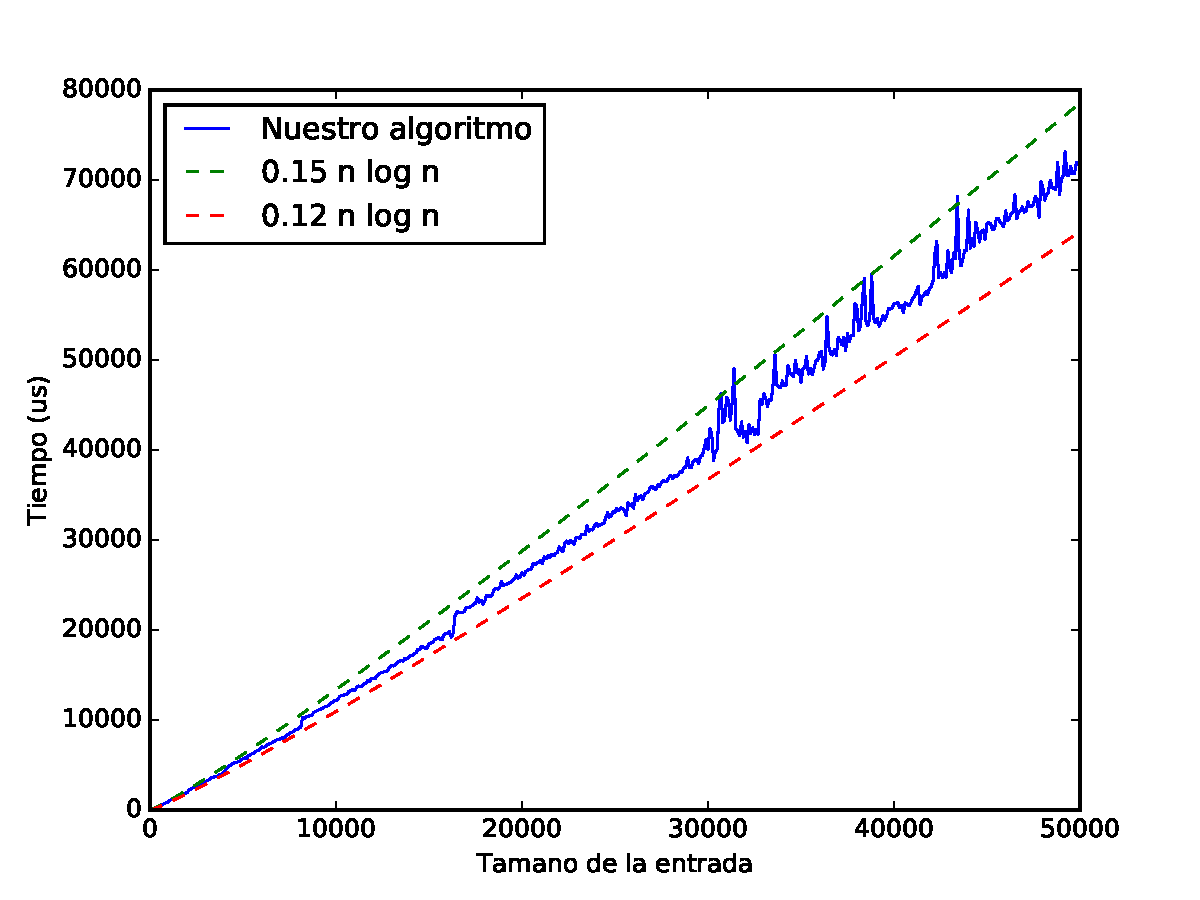
\includegraphics[width=0.8\textwidth]{img/tiempos/kaioken3.pdf}
	\caption{\footnotesize Tiempo que toma el algoritmo en $\mu$s para una entrada de tamaño $n$.}
	\label{fig:kaioken-tiempos3}
\end{figure}

Se ve claramente en la figura \ref{fig:kaioken-tiempos3} que el tiempo que toma el algoritmo esta acotado por arriba y por debajo por $k n \log n$ para algun $k$, es decir, el algoritmo es $\Theta(n \log n)$.

Para hacer un análisis más fino e interesante, es necesario hacer un \emph{close-up} y ver las complejidades de mas cerca.

\begin{figure}[H]
 \centering
	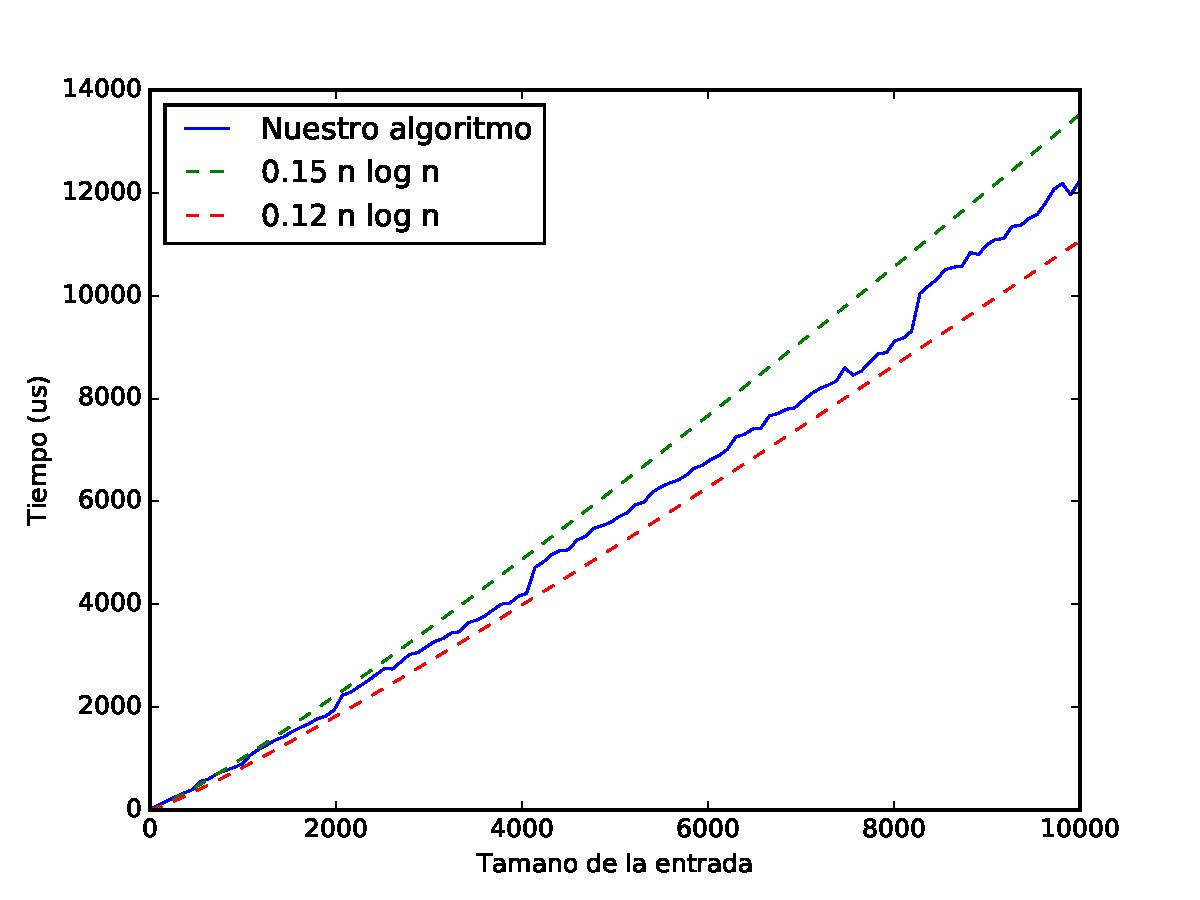
\includegraphics[width=0.8\textwidth]{img/tiempos/kaioken1.pdf}
	\caption{\footnotesize Tiempo que toma el algoritmo en $\mu$s para una entrada de tamaño $n$.}
	\label{fig:kaioken-tiempos1}
\end{figure}

Como puede verse en la figura \ref{fig:kaioken-tiempos1}, el algoritmo claramente es $\Theta(n \log n)$, pero también puede observarse que hay \emph{saltos} de tiempo en algunos lugares. Se puede inferir fácilmente que estos saltos suceden en las entradas donde $n = 2^k + 1$ para algun $k$, es decir, cuando $n$ es una potencia de 2 más 1. Esto se debe a que, como fue explicado antes, la cantidad de peleas necesarias es $\lceil \log_2(n) \rceil$, entonces para todos los numeros entre dos potencias de 2, la cantidad de peleas requerida es la misma, pero luego de una potencia de 2 esta cantidad de peleas aumenta en 1. A esto se debe los saltos luego de las potencias de 2.

Para visualizar más claramente este hecho, realizamos el siguiente gráfico, en el que están marcadas las potencias de 2.

\begin{figure}[H]
 \centering
	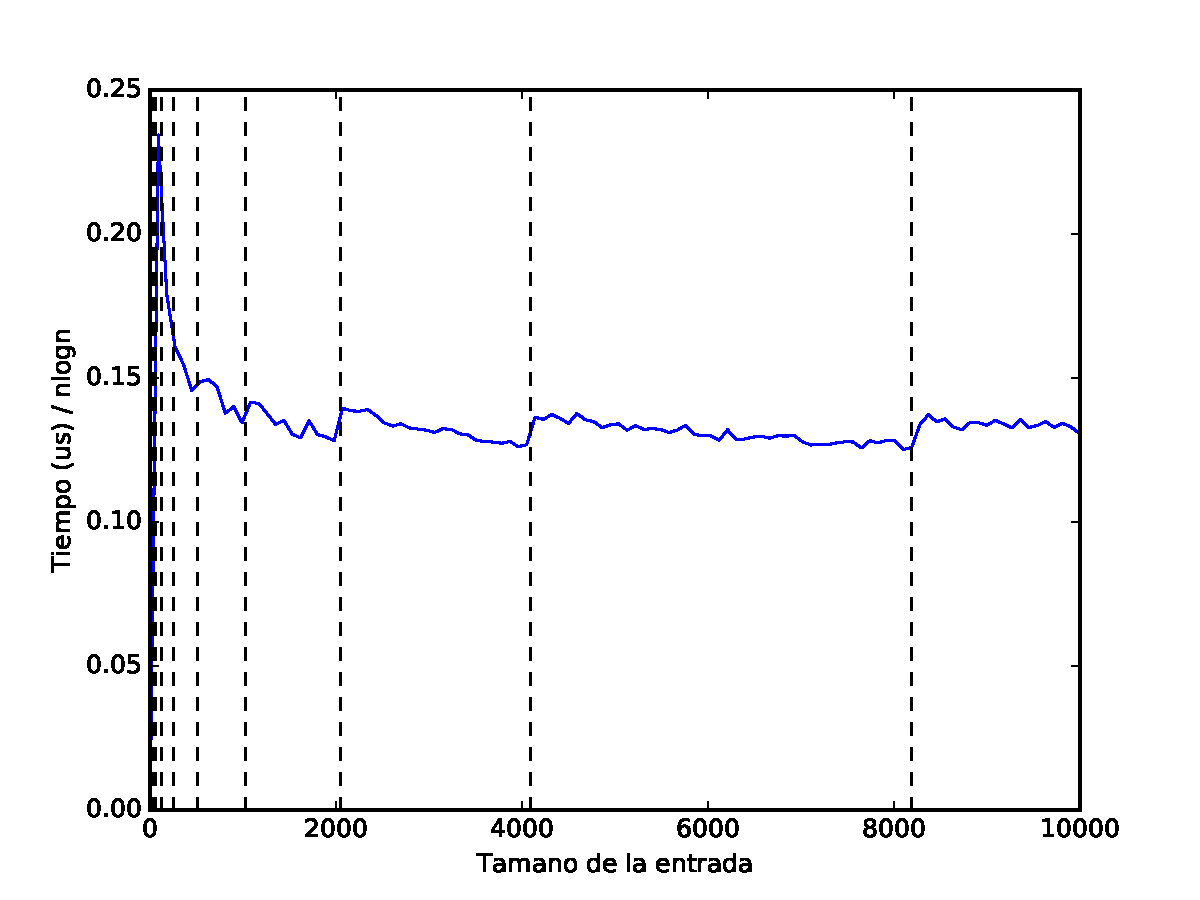
\includegraphics[width=0.8\textwidth]{img/tiempos/kaioken2.pdf}
	\caption{\footnotesize Tiempo que toma el algoritmo en $\mu$s dividido $n\log n$para una entrada de tamaño $n$.}
	\label{fig:kaioken-tiempos2}
\end{figure}

Con la figura \ref{fig:kaioken-tiempos2} se confirma lo que dijimos anteriormente. Luego de cada potencia de 2, el tiempo aumenta, y luego baja lentamente, dado que la relacion tiempo - $n \log n$ se mantiene constante, pero $n$ aumenta, con lo cual la división se achica.


\subsubsection{M\'etodo de experimentación}

Para este problema es fue muy fácil generar casos de prueba, dado que el único input para el programa es $n$, por lo que simplemente corrimos el programa con diferentes $n$ de entrada. Ejecutamos el programa 50 veces para cada $n$ y el resultado que graficamos fue el mínimo de todas las ejecuciones (para cada $n$). Elegimos el mínimo porque es el que nos permite eliminar outliers que tienen que ver con context switches o con factores de la ejecucion sobre los que no tenemos control.


